\documentclass{beamer}
\usepackage[utf8]{inputenc}
\usepackage[T1]{fontenc}
\usepackage[ngerman]{babel}
\usepackage{lmodern}
\usepackage{graphicx}
\usepackage{gensymb}
\usepackage{bold-extra}
\usepackage{textcomp}

\input{../flat-blue-theme.inc}

% Make \pause sections invisible
\setbeamercovered{invisible}
\newenvironment{fakt}[1]
{\begin{frame}{Fakt Nr. #1}\centering}
{\end{frame}}

%\newcommand{\rating}[1]{\\\hfill\\\pause Rating: #1/10}
\newcommand{\rating}[1]{}

\newcommand{\wiki}[1]{\\\hfill\\Wikipedia: #1}

\newcommand{\source}[1]{\\\hfill\\Quelle: #1}

%\title{Fakten}
%\subtitle{Oder: Irgendwelche random Dinge, die ich im Internet gelesen habe und die so klingen als könnten sie wohl stimmen.}
%\author{Hauke Stieler\\\href{mailto:4stieler@informatik.uni-hamburg.de}{4stieler@informatik.uni-hamburg.de}}
%\titlegraphic{
\includegraphics[width=1.5cm,keepaspectratio]{images/Openstreetmap-logo}}
%\date{27. Oktober 2020}

\begin{document}
	\begin{frame}
		\begin{center}
			{\huge Fakten}\\
			\hfill\\\pause
			Oder: Irgendwelche random Dinge, die ich im Internet gelesen habe und die so klingen als könnten sie wohl stimmen.
		\end{center}
	\end{frame}
	
	\begin{fakt}{1}
		"`We smell sausage"' klingt rückwärts ausgesprochen wie "`Jesus loves you"'.
		\rating{4}
		\source{Internet}
	\end{fakt}

	\begin{fakt}{2}
		Wenn man lächelt, drückt ein Muskel zwischen Wange und Auge auf einen Nerv, der im Gehirn Glücksgefühle auslöst.
		\rating{3}
		\source{Internet}
	\end{fakt}

	\begin{fakt}{3}
		Es gab 1962 in Tansania eine Lachepidemie, die dazu führte, dass Schulen geschlossen wurden. Rund 1000 Menschen waren über lange Zeit betroffen.
		\rating{7}
		\wiki{Tanganjika-Lachepidemie}
	\end{fakt}
	
	\begin{fakt}{4}
		Der Maintainer von "`less"' (dem GNU-Tool) heißt Mark Nudelman. \pause Mhhh ... \pause Nudeln ... \pause
		\rating{6}
		\wiki{Less\_(Unix)}
	\end{fakt}

	\begin{fakt}{5}
		Bei \texttt{grep} muss man manchmal sein Hirn einschalten, deswegen gibt es die Parameterfolge \texttt{-Hirn} um angenehm in Dateien zu suchen.
		\rating{10}
		\source{\texttt{grep} man-page}
	\end{fakt}

	\begin{fakt}{6}
		Die Lateinische Bezeichnung des Vogels "`Wachtelkönig"' ist "`Crex Crex"'. \pause
		Crex ist kein lateinisches Wort.
		\rating{8}
		\wiki{Wachtelkönig}
	\end{fakt}

	\begin{fakt}{7}
		"`Spermin"' gibt dem menschlichen Sperma Geschmack und Geruch, ist eigentlich fest und wird in Anti-Aging Produkten eingesetzt.
		\rating{8}
		\wiki{Spermin}
	\end{fakt}

	\begin{fakt}{8}
		Verschiedene Inhaltsstoffe von Sperma (u.A. Hormone wie Testosteron, Östrogen, Prolactin) können Antidepressiv wirken.
		\rating{9}
		\wiki{Sperma\#Antidepressive\_Wirkung}
	\end{fakt}
	
	\begin{fakt}{9}
		Nach GNU, Stallman, Linux, Torvalds und Berners-Lee wurden Asteroiden benannt (9965, 9882, 9885, 9793 und 13926).
		\rating{6}
		\wiki{u.a. Liste\_der\_Asteroiden}
	\end{fakt}
	
	\begin{fakt}{10}
		Der dritte Apple-Gründer (Ronald Wayne) hat nach 12 Tagen den Glauben an Apple verloren und seine 10\% Unternehmensanteile verkauft (heutiger Wert: über 230 Mrd. \$).
		\rating{10}
		\wiki{Ron\_Wayne}
	\end{fakt}
	
	\begin{fakt}{11}
		Eine Schleimschicht schützt Clownsfische vor den Nesselzellen der Anemonen. Den Schleim stellen sie nicht selbst her, sondern die Anemone und schützt so ihre Clownsfische <3\\
		\hfill\\
		Anemone und Clownsfisch lernen sich also erst kennen und wenn sie sich mögen, schützt die Anemone den Fisch mit Schleim.
		\rating{8}
		\wiki{Echter\_Clownfisch}
	\end{fakt}
	
	\begin{fakt}{12}
		Das Tupanvirus sieht aus wie Raumschiff Enterprise.\\\pause
		\hfill\\
		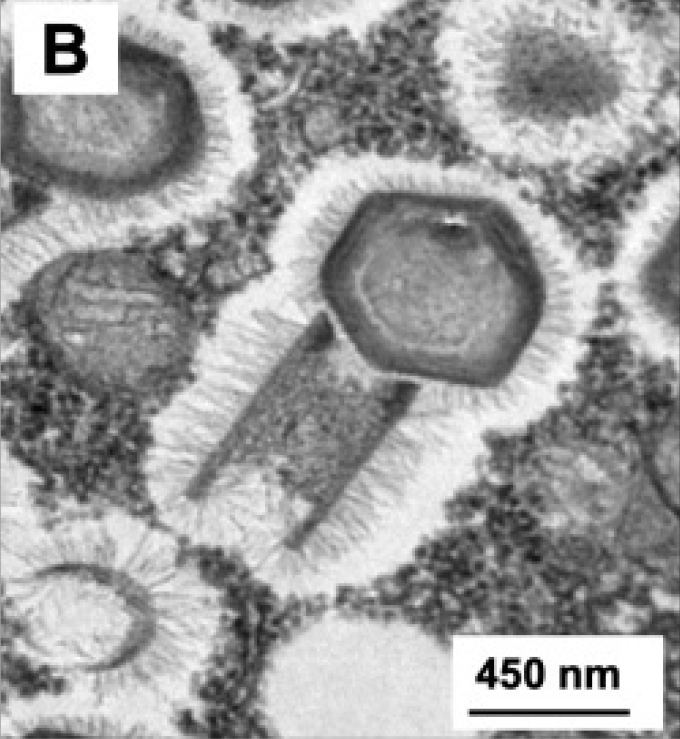
\includegraphics[width=4cm]{images/Tupanvirus}
		\rating{DS9}
		\wiki{Tupanvirus}
	\end{fakt}
	
	\begin{fakt}{13}
		Manche Spinnen bestehen zu 80\% aus Gehirn, was bis in die Beine reicht. Damit können selbst kleinste Spinnen komplexe Netze bauen.
		\rating{8}
		\source{National Geographic - "`Kleine Spinnen mit riesigen Gehirnen"'}
	\end{fakt}
	
	\begin{fakt}{14}
		Manche Spinnen fliegen indem sie dünne Fäden produzieren (ca. 320nm dick). Das klappt auch bei Windstille dank Termik oder minimaler elektrostatische Felder in der Luft.\\
		\hfill\\
		Schon Darwin beobachtete mitten auf dem Atlantik dieses Phänomen. Die meisten Spinnen sterben allerdings dabei.
		\rating{9}
		\wiki{Spinnenflug}
	\end{fakt}
	
	\begin{fakt}{15}
		Um den Juptermond "`Europa"' nicht mit irdischen Mikroorganismen zu kontaminieren, lies man die Raumsonde "`Galileo"' nicht auf Europa abstürzen, sondern steuerte sie in der Jupiteratmosphäre. Sie verglühte dann dort.
		\rating{10}
		\wiki{Galileo\_(Raumsonde)}
	\end{fakt}
	
	\begin{fakt}{16}
		Es gibt eine Tiefseequalle mit dem Namen "`flying spaghetti monster"' oder auch "`Bathyphysa conifera"', weil es sehr ans FSM erinnert. Es wurde während Wartungsarbeiten an einer Ölplatform entdeckt.\\
		\hfill\\
		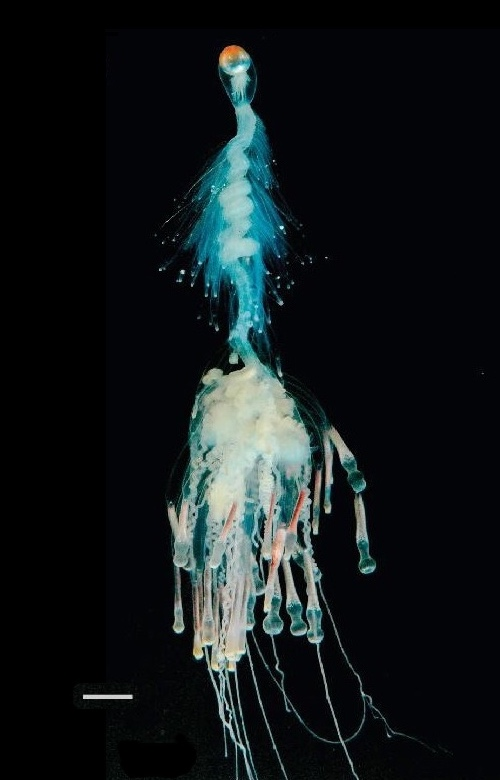
\includegraphics[width=2.5cm]{images/fsm}
		\rating{8}
		\wiki{Bathyphysa\_conifera}
	\end{fakt}
	
	\begin{fakt}{17}
		Der Pilz "`Ophiocordyceps sinensis"' befällt Raupen von innen nach außen.
		In Tibet ist er so beliebt, dass er als Zahlungsmittel benutzt wird.
		Preis / kg: 21.000 -- 43.000 Euro. Ist eine bedrohte Art und der begehrteste Parasit der Welt.\\
		\hfill\\
		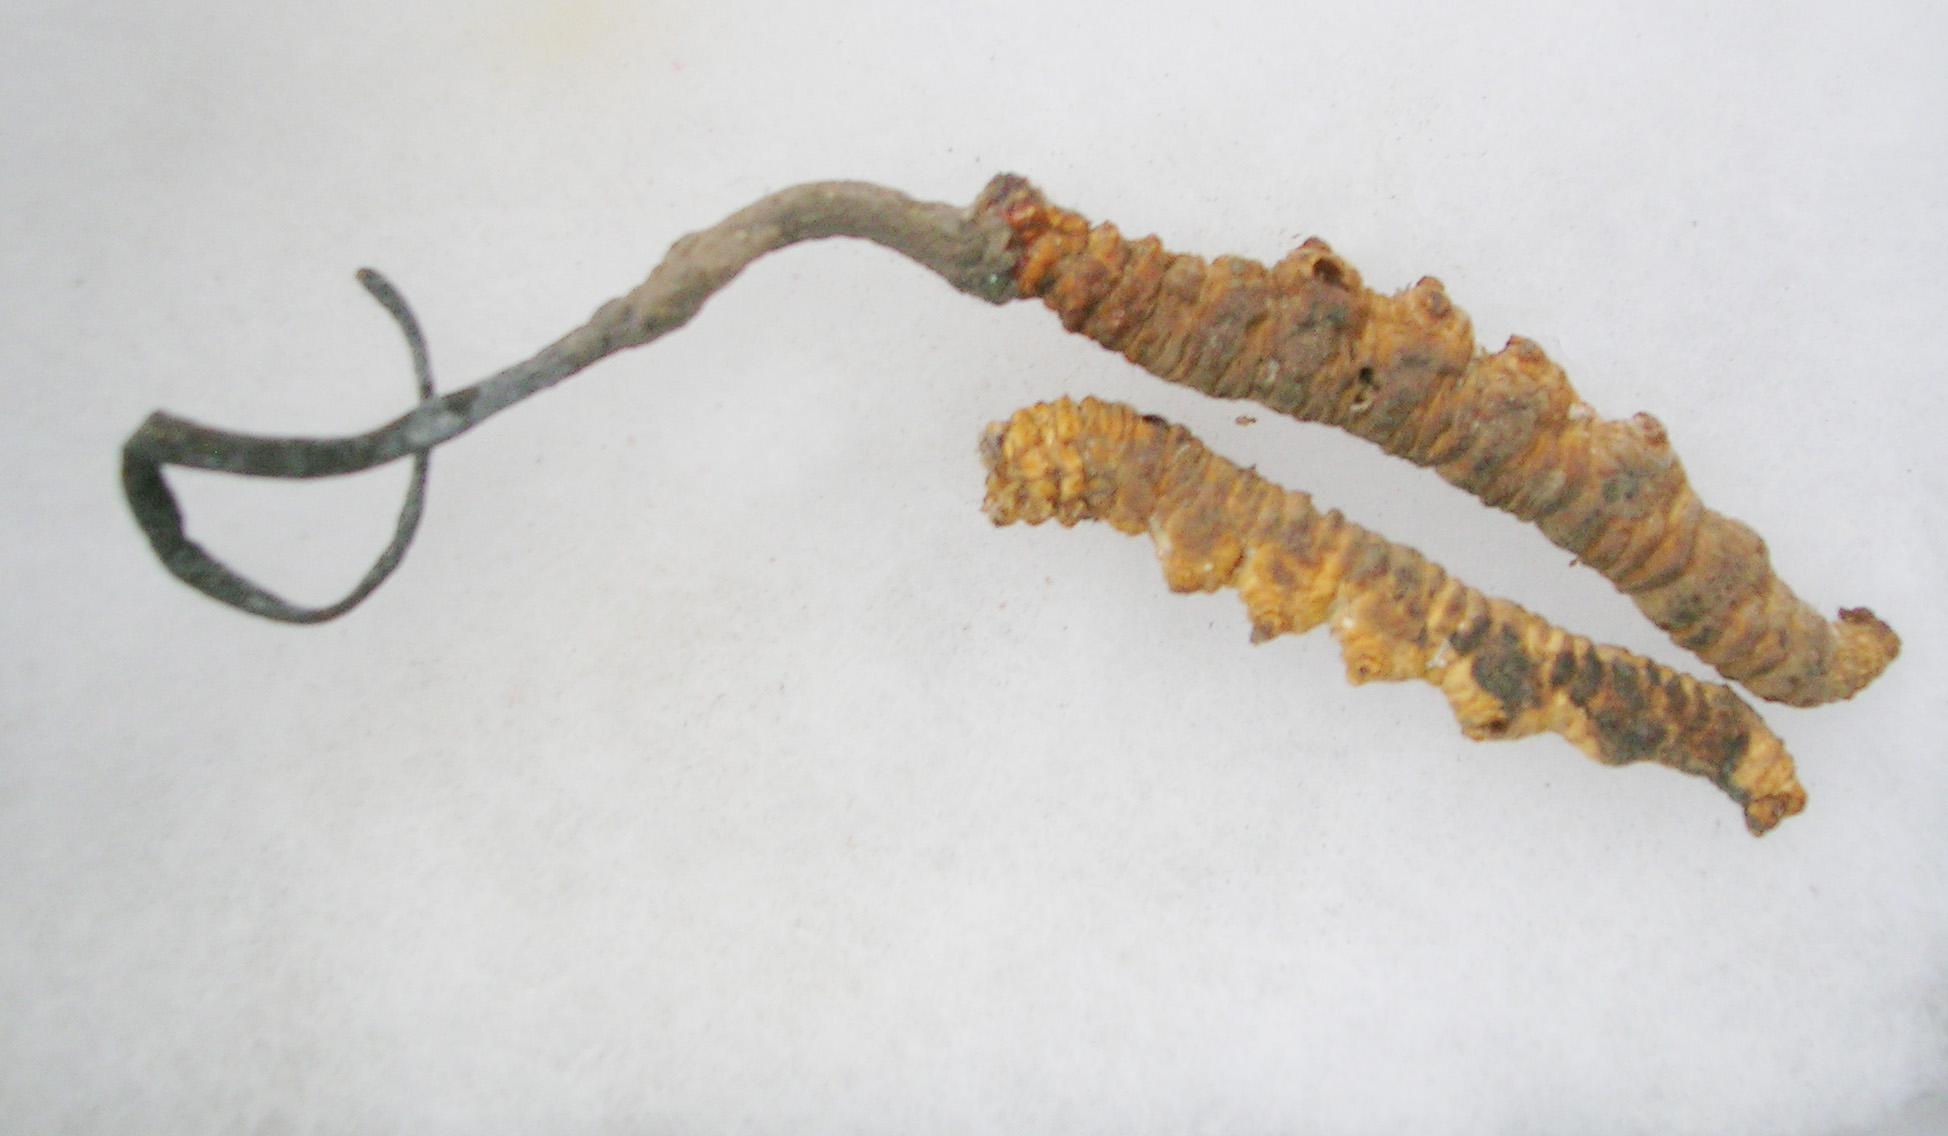
\includegraphics[width=5cm]{images/CordycepsSinensis}
		\rating{8}
		\wiki{Chinesischer\_Raupenpilz}
	\end{fakt}
	
	\begin{fakt}{18}
		Spongebobs Hausschnecke Gary heißt mit bürgerlichem Namen Garold Wilson Jr. und ist der Cousin von Patrick.
		\rating{11}
		\source{Spongepedia: Gary}
	\end{fakt}
\end{document}